% @Author: Your name
% @Date:   2017-08-17 15:16:16
% @Last Modified by:   Your name
% @Last Modified time: 2023-03-21 09:30:44
%%    2009/03/12 v1.0 GAUBM Vorlage f�r Aschlussarbeiten Physik
%% Template fuer Bachelor- und Masterarbeiten
%% an der Fakultaet fuer Physik (c) Thomas Pruschke der GA Universit�t
%% Verbesserungsvorschlaege bitte an studiendekanat@physik.uni-goettingen.de
%%
%% Benoetigte Pakete: datenumber
%%

%%%%%%%%%%%%%%%%%%%%%%%%%%%%%%%%%%%%%%%%%%%%%%%%%%%%%%%%%%%%%%%%%%%%%%
%%%%%%%%%% Bitte vor dem Veraendern diese Datei umbenennen! %%%%%%%%%%
%%%%%%%%%%%%%%%%%%%%%%%%%%%%%%%%%%%%%%%%%%%%%%%%%%%%%%%%%%%%%%%%%%%%%%

%% scrbook - Ersatz f�r LaTeX book Klasse aus dem KOMA Script
%% Moegliche Optionen: diejenigen der Klasse scrbook ausser titlepage

%% deutsche Arbeit:
\documentclass[bachelor,       %% Typ der Arbeit: bachelor oder master
               twoside,        %% zweiseitiges Layout
               BCOR10mm,       %% Bindekorrektur 10 mm
%               liststotoc,nomtotoc,bibtotoc, %% Aufnahme der div. Verzeichnisse
                                              %% ins Inhaltsverzeichnis
%               english,ngerman, %% Alternativspr. Englisch, Dokumentspr. Deutsch
                ngerman,english  %% Alternativspr. Deutsch, Dokumentspr. Englisch
%               final,          %% Endversion; draft fuer schnelles Kompilieren
               ]{GAUBM}

\usepackage{setspace}  %% Zur Setzung des Zeilenabstandes
\usepackage{babel}     %% Sprachen-Unterstuetzung
\usepackage{calc}      %% ermoeglicht Rechnen mit Laengen und Zaehlern
\usepackage[T1]{fontenc}       %% Unterstutzung von Umlauten etc.
\usepackage[latin1]{inputenc}  %% 
%% in aktuellem Linux & MacOS X wird standardmaessig UTF8 kodiert!
%\usepackage[utf8]{inputenc}    %% Wenn latin1 nicht geht ...

\usepackage{amsmath,amssymb} %% zusaetzliche Mathe-Symbole

\usepackage{lmodern} %% type1-taugliche CM-Schrift als Variante zur
                     %% "normalen" EC-Schrift
%% Paket fuer bibtex-Datenbanken
\usepackage[comma,numbers,sort&compress]{natbib}
\bibliographystyle{plainnat}

\newcommand{\tabheadfont}[1]{\textbf{#1}} %% Tabellenkopf in Fett
\usepackage{booktabs}                      %% Befehle fuer besseres Tabellenlayout
\usepackage{longtable}                     %% umbrechbare Tabellen
\usepackage{array}                         %% zusaetzliche Spaltenoptionen

%% umfangreiche Pakete fuer Symbole wie \micro, \ohm, \degree, \celsius etc.
\usepackage{textcomp,gensymb}

%\usepackage{SIunits} %% Korrektes Setzen von Einheiten
\usepackage{units}   %% Variante fuer Einheiten

%% Hyperlinks im Dokument; muss als eines der letzten Pakete geladen werden
\usepackage[pdfstartview=FitH,      % Oeffnen mit fit width
            breaklinks=true,        % Umbrueche in Links, nur bei pdflatex default
            bookmarksopen=true,     % aufgeklappte Bookmarks
            bookmarksnumbered=true  % Kapitelnummerierung in bookmarks
            ]{hyperref}

%% Weiter benoetigte Pakete: datenumber
%% Falls dieses Paket nicht in der Installation vorhanden ist,
%% kann es von der Seite mit diesem Template heruntergeladen werden
%% und in einem LaTeX bekanntem Verzeichnis installiert werden (notfalls
%% dem Verzeichnis mit der Arbeit).
\begin{document}
%%
%%                   Ab hier muessen die Anpassungen geschehen
%%
%% Hier den eigenen Namen einsetzen
\ThesisAuthor{Justus}{Multhaup}
%% Hier den Geburtsort einsetzen
\PlaceOfBirth{Boffzen}
%% Titel Arbeit. Das erste Argument ist der deutsche, das zweite der
%% englische Titel.
\ThesisTitle{Teilchensimulationen von Polymermischungen in begrenzten Geometrien mit zeitabh\"angigen Randbedingungen}{Particle simulations of polymer mixtures in confined geometries with time dependent boundary conditions}
%% Erst- und Zweitgutacher/in
%% Ist der/die Betreuer/in nicht identisch mit dem/r Erstgutachter/in,
%% muss diese/r als optionales Argument angegeben werden.
\FirstReferee{Prof. Dr. Marcus M\"uller}
\Institute{Institut f\"ur Theoretische Physik}
\SecondReferee{Prof. Dr. Stefan Klumpp}
%% Beginn und Ende des Anfertigungszeitraumes
\ThesisBegin{1}{4}{2009}
\ThesisEnd{15}{7}{2009}
%% DO NOT TOUCH THESE LINES!!!!
\frontmatter
\maketitle
\cleardoublepage


%% Ende des Vorspanns
\cleardoublepage
%% Ab hier 1 1/2 facher Zeilenabstand (durch setspace-Paket)
\onehalfspacing
%% Erzeugt Inhaltsverzeichnis
\tableofcontents

%% Hier kann man seine Bezeichnungsweisen erklaeren. Falls nicht
%% benoetigt, bis einschliesslich \end{nomenclature} auskommentieren
\begin{nomenclature}
%% Fuer die Berechnung der Spaltenbreiten muss \usepackage{calc}
%% geladen sein!
\section*{Lateinische Buchstaben}
\noindent
\begin{longtable}[l]{p{0.2\textwidth}p{0.7\textwidth-6\tabcolsep}p{0.1\textwidth}}
  \tabheadfont{Variable}&\tabheadfont{Bedeutung}&\tabheadfont{Einheit}\\\midrule\endhead
  $A$ & Querschnittsfl"ache & $\unit{m^2}$\\
  $c$ & Geschwindigkeit & $\unitfrac{m}{s}$
\end{longtable}
\section*{Griechische Buchstaben}
\begin{longtable}[l]{p{0.2\textwidth}p{0.7\textwidth-6\tabcolsep}p{0.1\textwidth}}
  \tabheadfont{Variable}&\tabheadfont{Bedeutung}&\tabheadfont{Einheit}\\\midrule\endhead
  $\alpha$  & Winkel & $\unit{\degree}$; --\\
  $\varrho$ & Dichte & $\unitfrac{kg}{m^3}$
\end{longtable}
\section*{Indizes}
\begin{longtable}[l]{p{0.2\textwidth}p{0.8\textwidth-4\tabcolsep}}
  \tabheadfont{Index}&\tabheadfont{Bedeutung}\\\midrule\endhead
  m & Meridian\\
  $r$ & Radial
\end{longtable}
\section*{Abk"urzungen}
\begin{longtable}[l]{p{0.2\textwidth}p{0.8\textwidth-4\tabcolsep}}
  \tabheadfont{Abk"urzung}&\tabheadfont{Bedeutung}\\\midrule\endhead
  2D & zweidimensional\\
  3D & dreidimensional\\
  max & maximal
\end{longtable}
\end{nomenclature}
%% \listoftables und \listoffigures sollten nur bei genuegender Anzahl Tabellen
%% verwendet werden
%\listoffigures
%\listoftables

\mainmatter   %% Anfang Hauptteil

\chapter{Introduction}


\chapter{Theory}

\section{Polymeric mixtures}

Polymer mixtures consist of two or more chemically different polymer types. The mechanical and thermodynamic properties can vary greatly with several factors such as composition, molecular weight and interactions between the polymers. This makes them desirable for manufacturing materials with tailored properties.\\
If the composition is uniform everywhere, then the mixture is called homogeneous. In this case, the properties do not change throughout the mixture. In a heterogeneous mixture, in contrast, the composition is non-uniform, leading to visible boundaries which may have very different properties. This phenomenon is also called macro-phase separation. From an entropic viewpoint, mixing is always favored. However, energetic interactions between polymers can either favor or suppress mixing. Whether a mixture is homogeneous or heterogeneous therefore depends on the balance between entropy and energy \cite[S. 137]{Rubin03}.           

\subsection{Flory Huggins Theory}

Whether mixing or phase separation will be favored can be predicted by determining the free energy change associated with mixing the components. This free energy change can be computed within the lattice model developed by Flory and Huggins \cite{Flory42}. Within the Flory-Huggins framework, no volume change is assumed upon mixing. With this assumption, it is convenient to represent the system on a lattice. The lattice site volume $v_0$ corresponds to the smallest molecular unit and every macromolecule takes up one or multiple lattice sites. Consider a binary mixture with $n_A$ polymers of species A and chain length $N_A$ and $n_B$ polymers of species B and chain length $N_B$. The free energy of mixing per lattice site $\Delta F_{mix}$ is then given by the Flory-Huggins equation of polymer solutions \cite[S. 143]{Rubin03}:

\begin{align}
  \frac{\Delta F_{mix}}{k_BT}=\frac{\phi}{N_A}\ln\phi+\frac{1-\phi}{N_B}\ln(1-\phi)+\chi\phi(1-\phi)\,.
\end{align}

Here, $\phi=\frac{n_AN_A}{n_AN_A+n_BN_B}$ is the monomer fraction of species A, $k_B$ is the Boltzmann constant, $T$ is the system temperature and $\chi$ is the Flory interaction parameter which characterizes the interaction between different polymer species and can be obtained from experiments. A positive value of $\chi$ opposes mixing while a negative value promotes it, knowing the value of $\chi$, therefore, allows a qualitative prediction of the phase separation behavior. Note that so far, no space dependence of $\phi$ has been assumed. To fully capture the complexity of the system, the Flory-Huggins model has to be extended to include spatial variations of $\phi$, which gives rise to the de Gennes-Flory-Huggins free energy functional  \cite{deGennes80, Reister02}:


\begin{align}
  \frac{F[\phi]}{k_BT}=\rho_0\int \mathrm{d}^3\mathbf{r}\left\{\frac{\phi}{N_A}\ln\phi+\frac{1-\phi}{N_B}\ln(1-\phi)+\chi\phi(1-\phi)+k(\phi)[\nabla\phi]^2\right\}\,.
  \label{eq:flory_fctl}
\end{align}

Here, $\rho_0$ is the average monomer density in the system. The term proportional to $[\nabla\phi]^2$ is added to the free energy density to ensure that unphysical, sharp changes in the local densities are penalized. The precise form of $k(\phi)$ depends on the strength of the parameter $\chi\,$. For $\chi N\ll 1\,,$ one considers the \textit{weak segregation limit} (WSL). For $\chi N\gg 1\,,$ the \textit{strong segregation limit} (SSL) is considered. For symmetric mixtures with $N_A=N_B=N\,,$ the prefactors $k$ take the form \cite{Reister02}:

\begin{align}
  k_{WSL}=\frac{R_e^2}{36N\phi(1-\phi)}\,;\qquad k_{SSL}=\frac{R_e^2}{18N\phi(1-\phi)}\,.
\end{align}


\section{Collective diffusion}

Consider a binary mixture of polymers with $N_A=N_B=N\,$. Since the number of monomers in the system is constant, the continuity equation holds:

\begin{align}
  \frac{\partial\phi}{\partial t}+\nabla\mathbf{J}=0\,.
  \label{eq:conti}
\end{align}

Here, $\mathbf{J}$ is the local current of species A. Near equilibrium, one postulates a linear relation between $\mathbf J$ and the local chemical potential difference $\mu$ \cite{deGennes80}:


\begin{align}
    \mathbf J(\mathbf{r})=-\int_V\frac{\Lambda(\mathbf{r}, \mathbf{r'})}{k_BT}\nabla '\mu(\mathbf{r'})\text d \mathbf{r'}\,.
    \label{eq:current}
\end{align}

The Onsager coefficient $\Lambda(\mathbf{r}, \mathbf{r'})$ relates the force acting on a monomer at position $\mathbf{r'}$ due to the gradient of chemical potential to the density at position $\mathbf{r}\,$. It therefore determines the dynamics of the system. For an incompressible symmetric mixture with $N_A=N_B=N\,$, in the simplest case, the current is coupled only locally to the chemical potential gradient. The Onsager coefficient then takes the simple form \cite{deGennes80, Binder83}

\begin{align}
  \Lambda=DN\phi(\mathbf{r'})(1-\phi(\mathbf{r'}))\delta(\mathbf{r}-\mathbf{r'})\,.
  \label{eq:onsager}
\end{align}

Here, $D$ is the single-chain diffusion coefficient.

\chapter{Simulation technique}
Text\dots

\chapter{Collective diffusion of symmetric homopolymers}

\section{Reference system}

In this section, the collective diffusion properties of noninteracting homopolymers with $N_A=N_B=N$ and $\chi=0$ are investigated. As a reference system, a simulation box with 10000 polymers and dimensions $L_x\times L_y\times L_z=9.25\times3\times3R_e^3$ is considered with a spatial discretization of $\Delta L=0.125R_e\,$, so the invariant degree of polymerization is $\sqrt{\bar{N}}\approx 120\,$. Periodic boundary conditions are applied in the lateral $y$ and $z$ directions, whereas impassable walls are applied in the $x$ direction. Initially, the polymers are distributed homogeneously in the system. To stimulate diffusion, conversion zones are introduced close to the walls at $x<0.25R_e$ and $x>9R_e\,$. In each time step, if the center-of-mass coordinate $\mathbf r_{cm}$ of a polymer of type A lies in the conversion zone at $x<0.25R_e\,$, it is converted to type B with probability $p(A\rightarrow B)=r\phi(\mathbf r_{cm})$ \cite{Dreyer22}. Analogously, conversion from B to A takes place in the conversion zone at $x>9R_e$ at the same rate $r\,$. The total currents $\mathbf{J_A}$ and $\mathbf{J_B}$ are measured by tracking the number of polymer conversions. 

\section{Collective diffusion coefficient}

It should be pointed out that the system can be described effectively in one dimension due to the periodic boundary conditions in the lateral directions and the equal conversion rates. The chemical potential is obtained by taking the functional derivative $\frac{\delta F}{\delta\phi}$ of \eqref{eq:flory_fctl}. Since $\chi=0\,$, no phase separation occurs and the local density differences are only caused by the dynamics. Assuming the WSL, the chemical potential becomes:


\begin{align}
  \frac{\mu}{\rho_0 k_BT}&=\frac{\ln\phi}{N}-\frac{\ln(1-\phi)}{N}-\frac{R_e^2}{18N\phi(1-\phi)}\frac{d^2\phi}{dx^2}\nonumber \\ &+\left[\frac{R_e^2(1-2\phi)}{36N\phi^2(1-\phi)^2}\right]\left(\frac{d\phi}{dx}\right)^2\,.
  \label{eq:flory}
\end{align}


\begin{figure}[h]
  \centering
  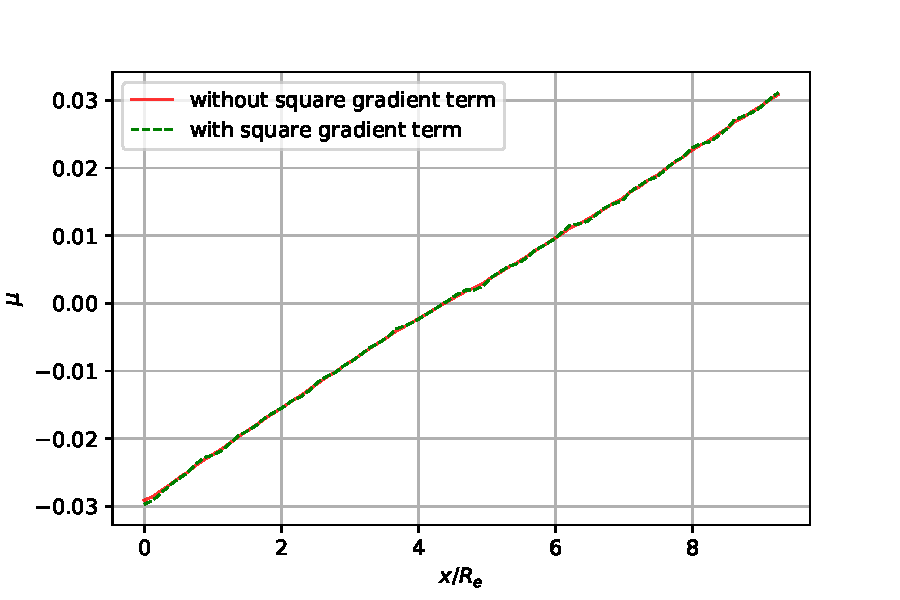
\includegraphics[width=0.5\linewidth]{figures/mu_coll_diff.pdf}
  \caption{Chemical potential with and without including the square gradient term in \eqref{eq:flory} for $r=0.0007$.}
  \label{fig:mu_coll_diff}
\end{figure}

In figure \ref{fig:mu_coll_diff}, it can be seen that the terms arising from the square gradient term do not contribute to the chemical potential and are therefore dropped from the following calculations for further simplification. From \eqref{eq:current}, the current of type A becomes:


\begin{align}
  J_A=-D\rho_0\frac{\partial\phi}{\partial x}\,.
  \label{eq:current_a}
\end{align}



Together with \eqref{eq:conti}, this gives the well-known diffusion equation:
\begin{align}
  \frac{\partial\phi(\mathbf r, t)}{\partial t}-D\rho_0  \frac{\partial^2\phi}{\partial x^2}=0\,.
  \label{eq:diffusion}
\end{align}

In the steady state, this simply yields $\frac{\partial^2\phi}{\partial x^2}=0\,$. Therefore, a linear density profile is obtained in the steady state. The slope is obtained from \eqref{eq:current_a} and the intersection is obtained from the condition that $\phi(L_x/2)=0.5$ since the density is normalized. 
\chapter{Discussion}
Text\dots
\chapter{Summary}
Text\dots

\appendix

\chapter{erster Anhang}


\cleardoublepage
%% Bibliographie. Das Argument muss der Name der BIBTeX-Datenbank stehen.
%% Ein Beispiel fuer eine solche Datenbank finden Sie in bthesis_datenbank.bib
\bibliography{bthesis_datenbank} 

\chapter*{Danksagung}
Dank\dots

%% Dieser Befehl MUSS am Ende stehen und erzeugt die Erklaerung ueber die
%% benutzten Mittel
\Declaration
\end{document}
